\
\begin{figure}[h]
\centering

\includegraphics[width=2cm]{NJTA.png}
\end{figure}
%============= Letter to New Jersey Turnpike Authority =
\section{Letter to New Jersey Turnpike Authority}
Dear Commissioners,\\
\\
Greetings!\\
\\
New Jersey Turnpike authority possesses the most heavily traveled toll roads in the whole US: New Jersey Turnpike (NJTP), and Garden State Parkway (GSP).\\ 
\\
They both have long history but are with high quality construction. NJTP was the third toll road in the nation and it opened in 1951, and now is a 14 lanes turnpike with 366 toll lanes at the 28 interchanges. GSP was opened in 1954, and has 12 lanes at its widest point, with 49 toll collection stations, 11 of them are toll plazas and 38 are on entrance or exit ramps [14].\\ 
\\
These two toll roads are very important for the US. In 2006, the average weekday daily transaction at the toll barrier can be as high as near 4500 during the AM peak period and over 3000 during the PM peak period, near 3000 during the peak period of weekends at the northbound [5]. Over 250 million vehicles used NJTP, that means there are over 690,000 vehicles per day on average [13]. With such heavy traffic flow, the bearing capacity of the toll plaza must be high.\\
\\
The tolling methods are very flexible at these toll roads. E-ZPass is an electronic toll collection system used in New Jersey. It can process 250 to 300 percent more vehicles than conventional manual tolling, which can reduce toll plaza delays and traffic congestion [12]. It makes the tolling event more efficient. E-ZPass was introduced to New Jersey in 1999 [5]. Now E-ZPass are acceptable on all lanes of NJTP and at the Pascack Valley, Raritan, Asbury, Toms River, Barnegat and Cape May Plaza of GSP. In 2014, 80\% of the tolls are collected by E-ZPass, and the proportion is still increasing [10]. Therefore, the efficiency of various tolling methods also needs to be seriously considered.\\
\\
We construct the model using multiple approaches, including queueing theory, stochastic distribution, guesstimation, and optimization under various circumstances. The model generates an input under the condition that every driver is rational that satisfies the queueing theory and can simulate the reality very well. We also offer a new shape of merge area that can cut the cost of road construction significantly, in the meantime, save the drivers' time wasted at the merging area.\\
\\
Notably, based on the fact of the common usage of E-ZPass and the heavy traffic flow in both toll roads, we also find out the most efficient arrangement of different categories of tollbooths and the toll plaza's performance under both light and heavy traffic flow.\\
\\
Hope our model helps!\\
\\
\noindent
best regards,\\
MCM

%============= Question Introduction ===================
\section{Introduction}
For the convenience of traveling, transportation construction rise from even the antiquity. However, it does cost the government lots of money to build and maintain the roads, bridges and so on. A toll road, also known as a turnpike or tollway, which is usually a public roadway where fee or toll is collected from every passenger to providing finance for the construction and maintenance of the roads. With its first major toll road built in 1790s, USA had over 5000 miles toll road constructed up till 2015.[5]\\
\\
Nonetheless, the cost of the government is solved though, the wasted time of travelers is increased due to the toll collection. To reach the win-win situation, the government should construct a suitable toll which costs both less money and time.

\subsection{Statement of the Problem}
There are two common tolls, one is ramp toll and the other is barrier toll. Every motorist should collect a card to enter the highway or pay the toll in order to leave the highway. According to the problem, the ramp tolls do not concern us here so we only consider the barrier tolls which is actually a row of tollbooths placed across the highway, perpendicular to the traffic flow.\\
\\
The number of tollbooths is usually larger than that of traffic lanes. Therefore, when leaving the tollbooths, vehicles must "fan in" from the larger number of traffic lanes to a relative small number of traffic lanes. In this problem, the fan-in-area is concerned in making the traffic model more efficient on both time consuming and cost.

\subsection{Assumption}
\begin{itemize}
\item
Motorists are all rational, which means they won't break any traffic rule, and all their driving behaviors are normal. Additionally, all drivers want to minimize their travel time, so they won't choose a longer queue when drive into the tollbooth area. Especially when all lines have the same number of vehicles, they won't change their line.
\item
The number of traffic lanes and the number of tollbooths of two directions are the same. Therefore, our model only consider one of the two opposite sides due to the symmetry.
\item
Assume it will take the same time for the drivers to be served at any tollbooth.
\item
There are two common ways of merging, one is merging from one side, cut down the number of traffic lanes until merging is completed. The other is merging from both side to the middle.
\\
\begin{figure}[h]
\small
\centering
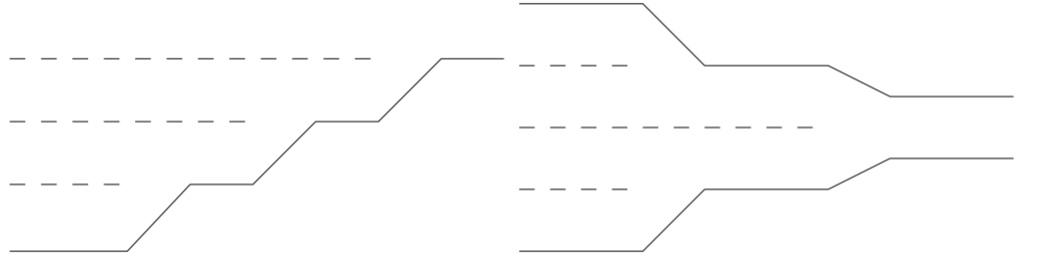
\includegraphics[width=12cm]{Two_Merging_Method.png}
\caption{Two Merging Methods} \label{fig:Two Merging Methods}
\end{figure}
\\
In the figure above, the number of traffic lanes decreases from 4 to 1. Although the number of traffic lanes cut down are the same in these two scenarios, the efficiency is different. In the second way, cars from two sides could begin "merging" at the same time, while cars in the first scenario could only merge from one lane to the neighbor lane one by one. Additionally, it is obvious that merging from one side costs more than merging from two sides. Therefore, in our model, the second method of merging is considered. 
\item
In the next section, we would assume that there's no self-driving(automated) car and all the tollbooths are of the same type. After the construction of the model, we will put the traffic situation, autonomous vehicles and different types of toll collection booths(human-staffed, exact-change and electronic tollbooths) into consideration to see how these factors affect our model.
\end{itemize}
\noindent
Under the above and basic assumptions, we can set out to construct our model (show our approach in detail).

%============ Question Analysis ========================
\section{Analysis of the Problem}
In this section, the problem will be divided into two parts and analysis will be done to help form the model.

\subsection{Gate Selection of Vehicles at Fan-out Area}
As mentioned before, all the tollbooths and vehicles are identical. We also assume that the queueing pattern at the tollbooths follows the first come first serve policy. Additionally, vehicles waiting in line are not allowed to renege, that is to leave or change the queue while waiting. So the motorist coming after is much more likely to choose the tollbooth with the shortest queue, that is with least vehicles waiting. Therefore, the vehicles tend to be distributed evenly at the plaza among all the tollbooths, and remain the pattern of even distribution while coming out of the tollbooths into the fan-in area since they all experience the same service time.

\subsection{Merging Pattern at Fan-in Area}
After toll, here comes a new stage: all vehicles set out at the speed of zero and merge at those merging points. Note that, since changes in flow occur smoothly and slowly, traffic flow(the number of vehicles in unit time) is usually considered to be roughly constant at any given moment. In other words, we could describe this process as a Poisson process where events happen continuously and independently at a constant average. Therefore, the traffic inter-arrival time must follow an exponential distribution before merging.[1]\\
\\
Given the roadway must narrow back from a number of tollbooth lanes to its normal width, common solutions used today are: 
\begin{itemize}
\item cut down the number of lanes from one side gradually
\item force a sharp merge at a relatively low speed
\end{itemize}
\noindent
Our solution to the problem will consider the fan-in shape which forces vehicles to merge from two side of the road to the middle, tending to minimize the waste time and construction cost.

%============= Construction of the model ===============
\section{Construction of the model}
\subsection{Queuing Theory}
Under our hypothesis, vehicles wait for the service of toll collection in tollbooths and may stop to waste time waiting for merging at the merging points. To model such process where customers line up to wait for service, we apply Queuing Theory.[2] It is common to use the symbols:
\begin{itemize}
\item $\lambda$ to be the mean or average number of arrivals per time period, i.e. the mean arrival rate.
\item $\mu$ to be the mean or average number of customers served per time period, i.e. the mean service rate.
\end{itemize}
We use notation system A/B/C to classify queuing model, where[2]
\begin{itemize}
\item A represents the probability distribution for the arrival process, which is also exponential distribution as we mentioned in the last section;
\item B represents the probability distribution for the service process, which is exponential distribution as we mentioned in the last section;
\item C represents the number of channels(servers), which is \# of tollbooths here.
\end{itemize}

\begin{table}[h]
\begin{center}
 \begin{tabular}{||c c c||} 
 \hline
 Characteristics & Symbols & Description \\ [0.5ex] 
 \hline\hline
 A & M & Exponential Distribution \\ 
 \hline
 B & M & Exponential Distribution \\
 \hline
 C & 1, 2 ... $\infty$ & Ideal Model \\
 \hline
 D & 1, 2 ... $\infty$ & Ideal Model \\
 \hline
 E & FCFS & First come fist serve \\ [1ex] 
 \hline
\end{tabular}
\caption{Queue System Parameters}
\label{table:1}
\end{center}
\end{table}

\noindent
In our model, it is M/M/C queuing system where M represents for a Poisson arrival distribution(exponential inter-arrival distribution) and C represents there are C tollbooths. By Burke's Theorem[3], the outcoming stream from the toll plaza also has the exponential distribution with the same rate as the arrival stream. This property will be used in the queue model of merging points.

\subsection{Merging Points and Process}
In the model, the number of traffic lanes decreases one after each merging point and all merging points are two-to-one merging points. For simplification, we assume that at the merging point, the vehicle on the main lane will drive first and the vehicle on the other lane will stop to wait if it cannot merge at that moment.

\subsection{Probability and Arrival Rate}
Consider the situation with L lanes and B tollbooths, where \(B, L \in \mathbb{N}\) and \(B\geqslant L\). We merge from both side by one lane simultaneously, so the total number of merging points at one side is \(\frac{B-L}{2}\) if \(B \equiv L \mod 2\), \(\frac{B-L-1}{2}\) on one side, \(\frac{B-L+1}{2}\) on the other side when \(B \equiv L+1 \mod 2\). However, at every merging point, arrival rate equals to the traffic flow it receives, so they are different among merging points.\\
\begin{figure}[h]
\small
\centering
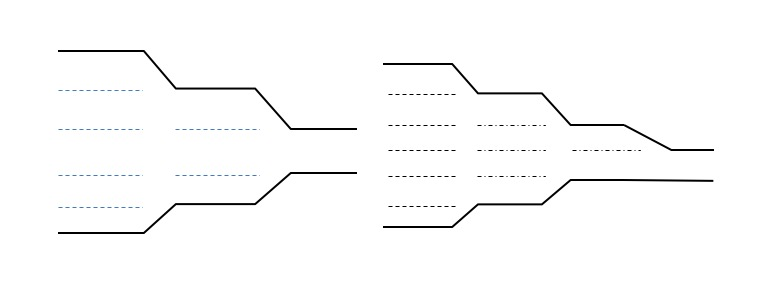
\includegraphics[width=12cm]{562831237.jpg}
\caption{Merging Model of Different B} \label{fig: Merging Model of Different B}
\end{figure}
\\
When  \(B \equiv L \mod 2\), the two sides are symmetric, so we may only consider one side.\\
\\
At the first merge point, the arrival rate is\\
\[
\lambda = \frac{2}{B} \times \phi
\]
since it bears the vehicles from the left-most two lanes.\\
\\
\noindent
At the second merge point, the arrival rate is\\
\[
\lambda = \frac{3}{B} \times \phi
\]
since it bears the vehicles from the left-most three lanes.\\
\\
So we may say that at the \(\frac{B-L}{2}\)-th merging point, the arrival rate is\\
\[
\lambda = \frac{B - \frac{B-L}{2}+1}{B} \times \phi
\]
When \(B \equiv L+1\mod 2\), the two sides are not symmetric. We may first consider merge from B tollbooths to (L+1) lanes. Then the method is the same as when \(B \equiv L \mod 2\), substituting L with (L+1). So at the \(\frac{B-L-1}{2}\)-th merging point, the arrival rate is\\
\[
\lambda = \frac{B-\frac{B-L-1}{2}+1}{B} \times \phi
\]
\\
There is still one merge point that will merge the (L+1) lanes to L lanes. So at this point, the arrival rate is\\ 
\[
\lambda = \frac{B-\frac{B-L+1}{2}+1}{B} \times \phi
\]

\section{Calculating and Simplifying the Model}
\subsection{Appearing Variables}
\begin{itemize}
\item Total Traffic Flow($\phi$). According to the Institute of Transportation Engineers[4], the maximum traffic flow of one lane is 2000/hour. Light and heavy traffic condition have different value of $\phi$. In New Jersey, the number of vehicles per lane per hour is 1300[5].
\item Service Rate at the Merging Point:
\begin{itemize}
\item No other cars: $\mu_{a}$. Since after getting into the highway, vehicles should speed up to at least 40 km/h. To prevent accident, the distance between two vehicles should be long enough. According two the two-second-rule, after the former vehicle passes one point, there would be at least 2 seconds for the second vehicle to pass that point. Thus we estimate the duration when one vehicle pass a merge point as approximately 2 seconds.\\
\[
\mu_{a} = \frac{3600}{2.0 s} = 1800/hr
\]
\item Merging Needed: $\mu_{b}$. To estimate the service rate when merging needed, we use the similar approach. Assume the merging occurs safely and efficiently, then the distance between two vehicles tends to be the safety distance, which is the length of the vehicle(speed is low in this scenario). From NJTA, 96\% of vehicles are cars and 4\% are trunks and buses, so we estimate the size of the car as 4.5 meters[5]. Therefore the average service time is approximately 3 seconds by uniformly accelerated linear motion.\\
\[
\mu_{b} = \frac{3600}{3 s} = 1200/hr
\]
\end{itemize}
\end{itemize}

\subsection{Wasting Time(W)}
Since the movement of thousands of vehicles and the merging process is random, and the future of the process could be predicted given the condition of the process now. In other words, the future state of the process could be independent of states at the past. Therefore, in our model, we view the merging process as a Markov process and merging points as Markov systems.[6]\\
\\
At any merging point, the state of the system is measured by the number of vehicles in the system. Here, we use $\Lambda$ to represent the arrival rate. For any vehicle coming to the merging point, if there is no vehicle ahead of it the service rate would be $\mu_{a}$ and $\mu_{b}$ otherwise as we assumed and calculated before. Let $P_{0}, P_{1}, P_{2}, ... , P_{n}$ represent the possibility for the system to contain 0, 1, 2, ..., n vehicles. The average wasting time would be calculated after the system reach the equilibrium, i.e. all state would possess a certain possibility.\\
\\
Under the conditions that[7]\\
\begin{itemize}
\item all states of the Markov chain communicate with each other (i.e., it is possible to go from each state, possibly in more than one step, to every state);
\item the Markov chain is not periodic (a periodic Markov chain is a chain in which, e.g., you can only return to a state in an even number of steps);
\item the Markov chain does not drift away to infinity,
\end{itemize}
For a merging point, when the system has no vehicle, there would be $\Lambda P_{0}$ vehicles coming into the system to make the state change from possessing 0 vehicle to possessing 1 vehicle and $\mu_{a} P_{1}$ vehicles getting out of the system to make the state change from possessing 1 vehicle to possessing 0 vehicles. At equilibrium, we have\\
\[
P_{0}\Lambda = P_{1} \mu_{a}
\]
When the system has 1 vehicle, besides its interaction with the system of state of possessing 0 vehicle, there would be $\Lambda P_{1}$ vehicles coming into the system to make the state change from possessing 1 vehicle to possessing 2 vehicles and $\mu_{b} P_{2}$ vehicles getting out of the system to make the state change from possessing 2 vehicles to possessing 1 vehicles. At equilibrium, we have\\
\[
P_{0}\Lambda + P_{2}\mu_{b} = P_{1} \mu_{b} + P_{1} \Lambda
\]
Likewise, when there is n vehicles($n \geqslant 2$) in the system, we have\\
\[
P_{n-1}\Lambda + P_{n+1}\mu_{b} = P_{n} \mu_{b} + P_{n} \Lambda
\]
at the equilibrium. Besides summation property of possibility $P_{0} + P_{1} + P_{2} + \cdots + P_{n} = 1$, we obtain\\
\begin{empheq}[left=\empheqlbrace]{align}
P_{0} = (1 + \frac{\Lambda}{\mu_{a}} + \frac{2\mu_{b}\Lambda^2}{\mu_{a}(\mu_{a}+\Lambda)(\mu_{b}-\Lambda)})^{-1}\\
P_{1} = \frac{\Lambda}{\mu_{a}}\cdot P_{0}\\
P_{n} = \frac{2\Lambda^2}{\mu_{a}(\mu_{a}+\Lambda)} \cdot \frac{\Lambda}{\mu_{b}^{-2}}\cdot P_{0}, n \geqslant 2
\end{empheq}
\noindent
\\
Therefore, the average wasting time at a particular merging point could be calculated given the arrival rate and expected number of vehicles.
\[
w(\Lambda) = \lim_{n\to\infty} \frac{\sum_{i=0}^{n} iP_{i}}{\Lambda}
\]
With the knowledge of arrival rate $\lambda$ of each merging point and the possibility of reaching a merging point($\frac{\lambda}{\phi}$) calculated in section 4, when B-L is even, the total average wasting time at all merging points is
\[
W = 2\times\sum_{i=1}^{\frac{B-L}{2}} \frac{i+1}{B} \times w(\frac{i+1}{B}\cdot\phi)
\]
When B-L is an odd number.
\[
W = \sum_{i=1}^{\frac{B-L-1}{2}} \frac{i+1}{B} \times w(\frac{i+1}{B}\cdot\phi) + \sum_{i=1}^{\frac{B-L+1}{2}} \frac{i+1}{B} \times w(\frac{i+1}{B}\cdot\phi)
\]

% Here we need to add a graph to show the average wasting time
% L = 1, mu_a = 2160/hr, mu_b = 1200/hr
\begin{figure}[h]
\small
\centering
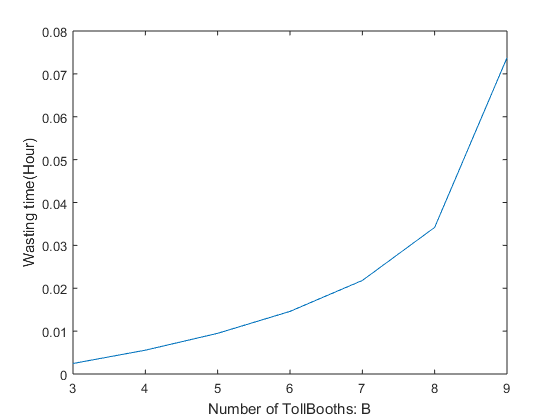
\includegraphics[width=12cm]{wasting_time.png}
\caption{Average Wasting Time When L = 2} \label{fig: Average Wasting Time when L = 2}
\end{figure}

\subsection{Construction Cost(C)}
The construction and maintenance fee of highway road is expensive, to minimize the cost, the government should build optimal and suitable roads. In this section, we will see how much the model cost. According to NJDOT, it costs about 335.7 USD per square meter to construct, maintain and administer the highway.[8]\\
\\
In our model, the merging process is going on at the same time on the two sides. At each merge point, there is a piece of "merging area" shown in figure 4. There would be totally $B-L$ merging area in the model. If $B-L$ is even number as the figure shows, there would be $\frac{B-L}{2}$ pairs of merging area. Otherwise, there would be $\frac{B-L-1}{2}$ pairs with one isolated merging areas.\\

\begin{figure}[h]
\small
\centering
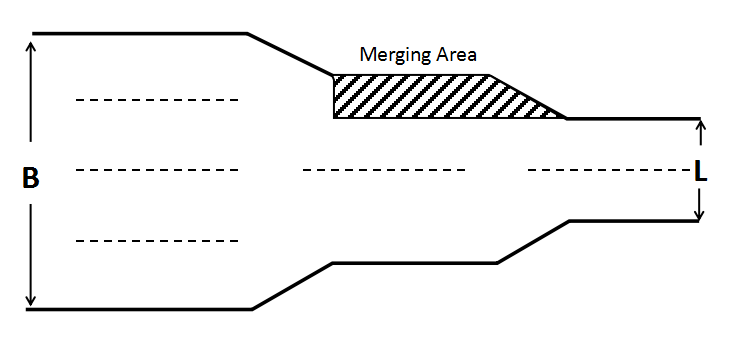
\includegraphics[width=12cm]{Merging_Area.png}
\caption{Merging Area} \label{fig: Merging Area}
\end{figure}
\noindent
At each merging area, the distance should be at least safety distance, which is 6 times car size. As we estimated before, the distance D is $6\times 4.5 = 27$ meters. Practically, the triangle part of merging area is at least the size of one vehicle which is 4.5 meters. The width of a traffic lane is 3.7 meters. Thus the area of one merging area is 108.225 $m^2$. If there are B tollbooths and L traffic lanes, the total cost would be\\
\[
C = [\ceil {\frac{B-L}{2}} \times L \times D \times 3.7 + (B-L)\times 108.225]\times 335.7
\]
\noindent
When L equals 2, the cost function of B is shown in figure 5.
% Add a figure to show the cost-B growth
\begin{figure}[h]
\small
\centering
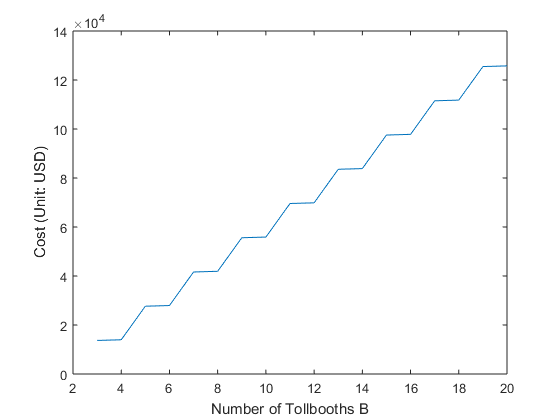
\includegraphics[width=12cm]{cost.png}
\caption{Highway Cost When L = 2} \label{fig: Highway Cost when L = 2}
\end{figure}

%========== 模型的实效分析(适应性说明)======================
\section{Validating the Model}
In this section, we will see how some certain factors affect our model.

\subsection{Light or Heavy Traffic}
In previous part, what we considered is under average traffic flow. What would our model behaves and give to us under various traffic condition? For instance, let us see Asbury Park Toll Plaza - Garden State Parkway whose B equals 4 and L equals 2. Below is the figure showing the change of wasting time with the change of traffic flow.\\

\begin{figure}[h]
\small
\centering
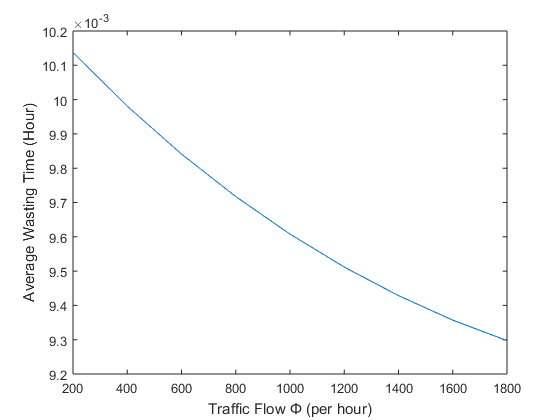
\includegraphics[width=12cm]{phi.png}
\caption{Average Wasting Time With Traffic Flow Changing} \label{fig: Average Wasting Time With Traffic Flow Changing}
\end{figure}
\noindent
From the figure, we see that the average wasting time during merging decreases slightly from 10.15$\times 10^{-3}$ to 9.3$\times 10^{-3}$ as traffic flow $\phi$ increases from 200 to 1800 per hour, which shows that if the traffic flow is in a reasonable range, it would not be a great effect on wasting time.

\subsection{Autonomous Vehicles}
Autonomous vehicles are more and more mature these years, new technologies make it safer, faster and more agile than human drivers. First, they may reduce the number of accidents caused by human error, such as being distracted and fatigue driving. Also, they can sense the environment rapidly and accurately with broad range of sensors, also, advanced GPS and operation-computing technology allow it to make accurate reactions to various environments.[9] Thus, the reaction time is reduced and the safety distance is also shorter than human drivers with the same velocity. That is to say, they require a higher speed limitation than human drivers.\\
\\
With a shorter reaction time, $\mu_{b}$ is smaller for the autonomous vehicles since it is the time for a car to drive through the merging area from the speed of 0. The difference between reaction time of human driver and automatic vehicle is roughly 0.2 second, which is obtained by estimation. Therefore, for autonomous vehicles,\\
\[
\mu_{c} = \frac{3600}{\frac{3600}{\mu_{b}} - 0.2} \approx 1300
\]
Meanwhile, $\mu_{a}$ remains the same since it is the time for a car to drive through the merging area at the average highway speed. The merging area and average speed are same for all vehicles, so $\mu_{a}$ remains unchanged.\\
\\
In a word, the autonomous vehicles only affect $\mu_{b}$. We set the proportion of the autonomous vehicle to be $a$, then the new service rate at merging point when merging occurs is\\
\[
\mu_{b}\prime = a\cdot\mu_{c} + (1-a)\cdot\mu_{b} = 100\cdot a + 1200
\]
When L equals 2 and B equals 4, the average wasting time changes with the proportion $a$ as\\
\begin{figure}[h]
\small
\centering
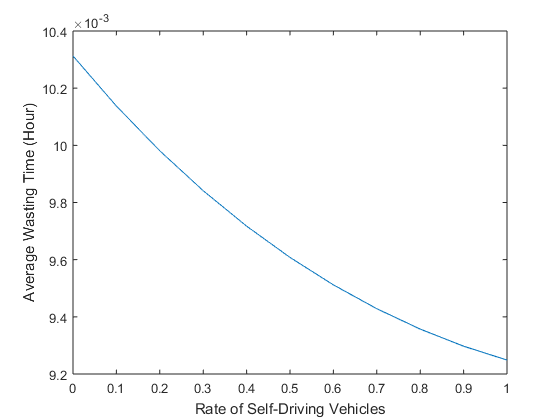
\includegraphics[width=12cm]{avg_sd.png}
\caption{Average Wasting Time With Self-Driving Vehicles Considered When L = 2, B = 4} \label{fig: Average Wasting Time With Self-Driving Vehicles Considered When L = 2, B = 4}
\end{figure}

\subsection{Conventional, Automated or Electronic Tollbooths}
There are various ways to collect toll in real life. Exact-change tollbooths and electronic toll collection (ETC) are also widely used other than the conventional manual tollbooths. These toll collection methods are all widely used. According to New Jersey Turnpike Authority, the usage of E-ZPass, the name of their ETC system, has reached 80.0\% in 2014, and remain slightly increasing.[10]\\
\\
The service rate of these three categories are different. We first define that the service rate of conventional manual tollbooth is the number of vehicles passing through the tollbooth in a unit time period, denoted by $\theta_{1}$(We estimate it as 350 per hour). Similarly, we also define the service rate of exact-change tollbooths $\theta_{2}$, the service rate of ETC $\theta_{3}$.\\
\\
According to NJTA design manual, the size of the tollbooths is around 40 feet[11]. We estimate the speed passing through the ETC to be 10 miles per hour. Therefore, we conclude that\\
\[
\theta_{3} = \frac{3600s}{40feet/10mph} = 1302/hour
\]
The service time of exact-change tolling is around a half of conventional manual tolling, the speed limit is the same as the speed going through ETC. Thus for exact-change tolling,\\
\[
\theta_{2} = \frac{3600s}{\frac{1}{2}(\frac{3600s}{\theta_{2}}-\frac{1}{\theta_{3}})+\frac{1}{\theta_{3}}} = 550 /hour
\]
Since service rate mainly affects the traffic flow of each tollbooths, $\phi$ is the only parameter that will be changed with the category of tolling methods

\subsubsection{Discussion on the Layout of Different Types of Tollbooths}
From the results we calculated in the last section, the service rates of conventional and automated tollbooths are more or less the same while the service of ETC is far more efficient. In this part, we will discuss how the layout of ETC, denoted by E afterwards, and normal tollbooth, denoted by N afterwards, affect the total wasting time of the system and whether there is a better merging pattern.\\  
\\
In our assumptions for the model, we view all merging process at merging points as two-to-one merging. And for simplification, we actually view two lanes as one queue waiting for merging. Therefore, there are three kinds of merging scenario with respect to types of tollbooth vehicles use: E to N, E to E, N to N. Since the motion of vehicles is complicated to simulate, we could not figure out which one would be less time consuming. In other words, it is hard to tell whether E to E + N to N is greater than 2 $\times$ E to N.\\
\\
To determine a better layout, we consider the case with $B = 6, L = 2$. Intuitively, the middle two lanes should be ETC lanes since vehicles passing through ETC are faster and the process is more efficient. With 80\% vehicles installed ETC, it could save much total average wasting time. Then there are two more cases to compare:\\
\begin{figure}[h]
\small
\centering
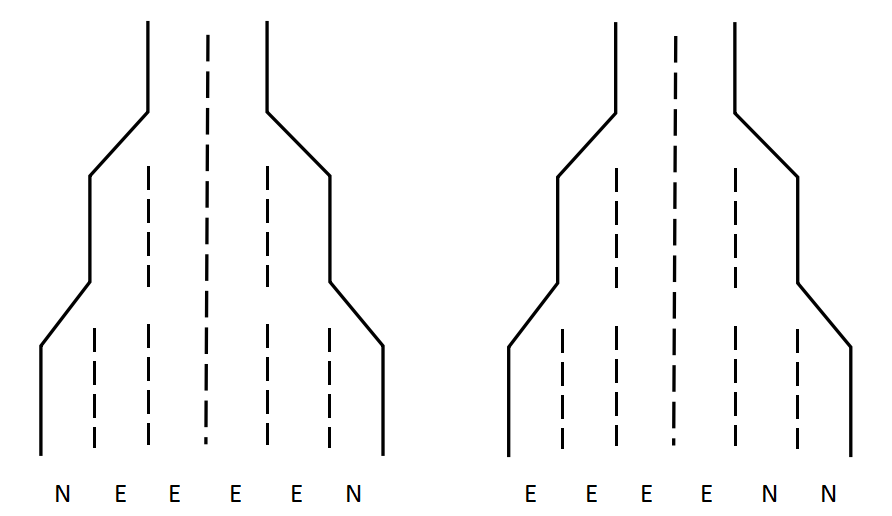
\includegraphics[width=12cm]{Layout.png}
\caption{Two Types of Layouts} \label{fig: Two Types of Layouts}
\end{figure}

\subsubsection{Wasting Time of Two Layouts: E/E/E/E/N/N or N/E/E/E/E/N?}
As the E lane has traffic flow 1302/hour and N lane has traffic flow 400/hour, by applying our model, the wasting time at a particular merging point is:
\[
w = \frac{1}{\mu_{b}-\Lambda} + \frac{\mu_{b}-\mu_{a}}{\Lambda(\mu_{b}-\mu_{a}) + \mu_{a}\mu_{b}} = \frac{1}{12-\Lambda} + \frac{1}{\Lambda-3600},
\]
where $\Lambda$ is the arrival rate at the merge point. Therefore, for the layout E/E/E/E/N/N, $\Lambda$ at four merging points are $\frac{1}{3}\times 1302, \frac{1}{2}\times 1302, \frac{1}{3}\times 400, \frac{1}{3}\times 400+\frac{1}{6}\times 1302$ respectively. For the layout N/E/E/E/E/N, $\Lambda$ at four merging points are $\frac{1}{6}\times 1302+\frac{1}{6}\times 400, \frac{1}{3}\times 1302+\frac{1}{6}\times 400, \frac{1}{6}\times 1302+\frac{1}{6}\times 400, \frac{1}{3}\times 1302+\frac{1}{6}\times 400$. The average wasting time of E/E/E/E/N/N is\\
\[
W_{1} = \sum\frac{\Lambda_{i}}{\phi}\cdot w(\Lambda_{i}) = 4.70556\times10^{-3} (hr)
\]
The average wasting time of N/E/E/E/E/N is\\
\[
W_{2} = \sum\frac{\Lambda_{i}}{\phi}\cdot w(\Lambda_{i}) = 4.6768\times10^{-3} (hr)
\]
Hence, N/E/E/E/E/N layout is less time-wasting compared to E/E/E/E/N/N layout.

%============ 总体评价 ====================================
\section{Evaluation: Strengths and weaknesses}
Like any model, our model presented above has its strengths and weaknesses. Some of the major points are presented below.

\subsection{Strengths}
\begin{itemize}
\item With rational analysis of the problem in the first place, we set up several assumptions to simplify the complicated question to fit in the Queuing Theory and also be relatively consistent with reality situation.
\item Our model is quite considerate since it incorporates various factors including size, cost of construction of the fan-out area, the merging pattern of the cars at first. Moreover, it also provides the further refinement with consideration of different kinds of tollbooths, proportion of self-driving cars and the layout of the tollbooths.
\item And with data coming from real world, we make sure the model keeps consistent with the practical situation by calculating our parameters based on realistic data.
\item Our model is quite understandable. Since it constructs the basic Queuing Model framework in the beginning with fundamental idea behind it elaborated and then take more complicated factors into consideration to make it more complete.
\end{itemize}

\subsection{Weakness}
\begin{itemize}
\item In our model, we does not consider irrational drivers. Without assuming all motorists are rational, the performance of toll could be less efficient, since some drives choose a long queue when waiting or speed up to bypass a car which causes traffic congestion. However, the possibility of such cases is so small that it could only cause minor change to the result.
\item When calculating the construction cost of our model, we does not consider the difference between splitting roads from two directions before merging and combining two together after merging.(Because if merge from two sides would lead to extra space in the middle.)
\item For simplification, at the merging points, we model the process as a two-to-one model. In other words, at any merging point, there are two lanes of vehicles queuing in one line to merge into one lane at the end. Since the actual motion of vehicles at the merging points is really complicated and every driver vary with each other, the model may not reflect actual condition correctly.
\item To introduce the stochastic process into our model, we assume the merging rate is constant once there are over 2 cars in the system. Although it should works well for under average traffic situation, it may cause error under extreme light or extreme heavy traffic conditions since the merge pattern under such situation could be different. In extreme light cases, for an example, the number of cars in a merge point is 2, they just change to different lanes and rush through without affecting each other. In the extreme heavy traffic conditions, there are maybe congestion everywhere including the merge point. So there maybe extra delay in such cases. However, each case is rare to happen in the reality and we need enormous amount of calculation to analyze them quantitatively, which is quite time-consuming and could not be done within the contest period.
\end{itemize}

\section{Conclusions}
How to minimize the wasting time of travelers at toll plaza and make the highway construction and maintenance fee optimized have always been a hot research direction for many years. However, to simulate the actual motion of vehicles may not be possible. Based on lots of research paper, our model simplify the problem by making reasonable assumptions and conclude several results efficiently. Merging from two sides could save construction cost. When the number of tollbooths is greater than the number of traffic lanes, wasting time in fan-in area would increase with the ascent of the number of tollbooths. In the reasonable traffic flow range, average wasting time is decreasing slightly. With more and more autonomous cars, wasting time could be deduced. When there are both ETC and normal tollbooths, setting ETC all at the middle is the more efficient way. Nonetheless, more test, simulation and improvement should be done in the future to make the model better before using the model practically in the real world.

\begin{thebibliography}{99}
\raggedright
\bibitem{1} Modeling Toll Plaza Behavior Using Queuing Theory. 2005. Retrieved from http://www.math.washington.edu/~morrow/mcm/cary05.pdf
\bibitem{2} Queuing Theory. J. E. Beasley. Retrieved from http://people.brunel.ac.uk/~mastjjb/jeb/or/queue.html
\bibitem{3} Burke's Theorem and Networks of Queues. M.I.T. Retrieved from https://ocw.mit.edu/courses/electrical-engineering-and-computer-science/6-263j-data-communication-networks-fall-2002/lecture-notes/Lecture7.pdf
\bibitem{4} Institute of Transportation Engineers, Traffic Engineering Handbook, Ed. James L. Pline, Prentice Hall, Englewood Cliffs, NJ, 1992.
\bibitem{5} Road User Cost Manual. New Jersey Turnpike Authority. Retrieved from http://www.state.nj.us/turnpike/documents/NJTA\%20Road\%20User\%20Cost\%20Manual.pdf
\bibitem{6} Markov Chains. James. N. Cambridge. Retrieved from http://u.math.biu.ac.il/~amirgi/CLN.pdf
\bibitem{7} Markov Chain and Markov Process. Retrieved from http://www.win.tue.nl/~iadan/sdp/h3.pdf
\bibitem{8} The Cost of Roadway Construction, Operations and Maintenance in New Jersey. 2016. Jon Carnegie, AICP/PP. Retrieved from http://www.state.nj.us/transportation/refdata/research/reports/NJ-2016-003.pdf
\bibitem{9} Self-Driving Car Technology’s Benefits, Potential Risks, and Solutions. 2014. John. M. Retrieved from $http://www.theenergycollective.com/jemiller_ep/464721/self-driving-car-technology-s-benefits-potential-risks-and-solutions$
\bibitem{10} E-ZPASS Usage. New Jersey Main Customer Service Center. Retrieved from $https://www.ezpassnj.com/en/about/i_guide.pdf$
\bibitem{11} Section 11: Facility Building and Toll Plaza. NJTA. Retrieved from http://www.state.nj.us/turnpike/documents/NJTA-DM-Section-11-Facility-Buildings-Toll-Plazas.pdf
\bibitem{12} NJ E-ZPass. Retrieved from https://www.ezpassnj.com/en/about/about.shtml
\bibitem{13} New Jersey Traffic and Revenue Study. NJTA. 2008. Retrieved from http://www.njslom.org/njtrstudypart2.pdf
\bibitem{14} New Jersey Turnpike Authority Website. Retrieved from http://www.state.nj.us/turnpike/who-we-are.html
\end{thebibliography}